\documentclass{standalone}
\usepackage{tikz}
\usepackage[outline]{contour}
\begin{document}
\contourlength{0.2em}
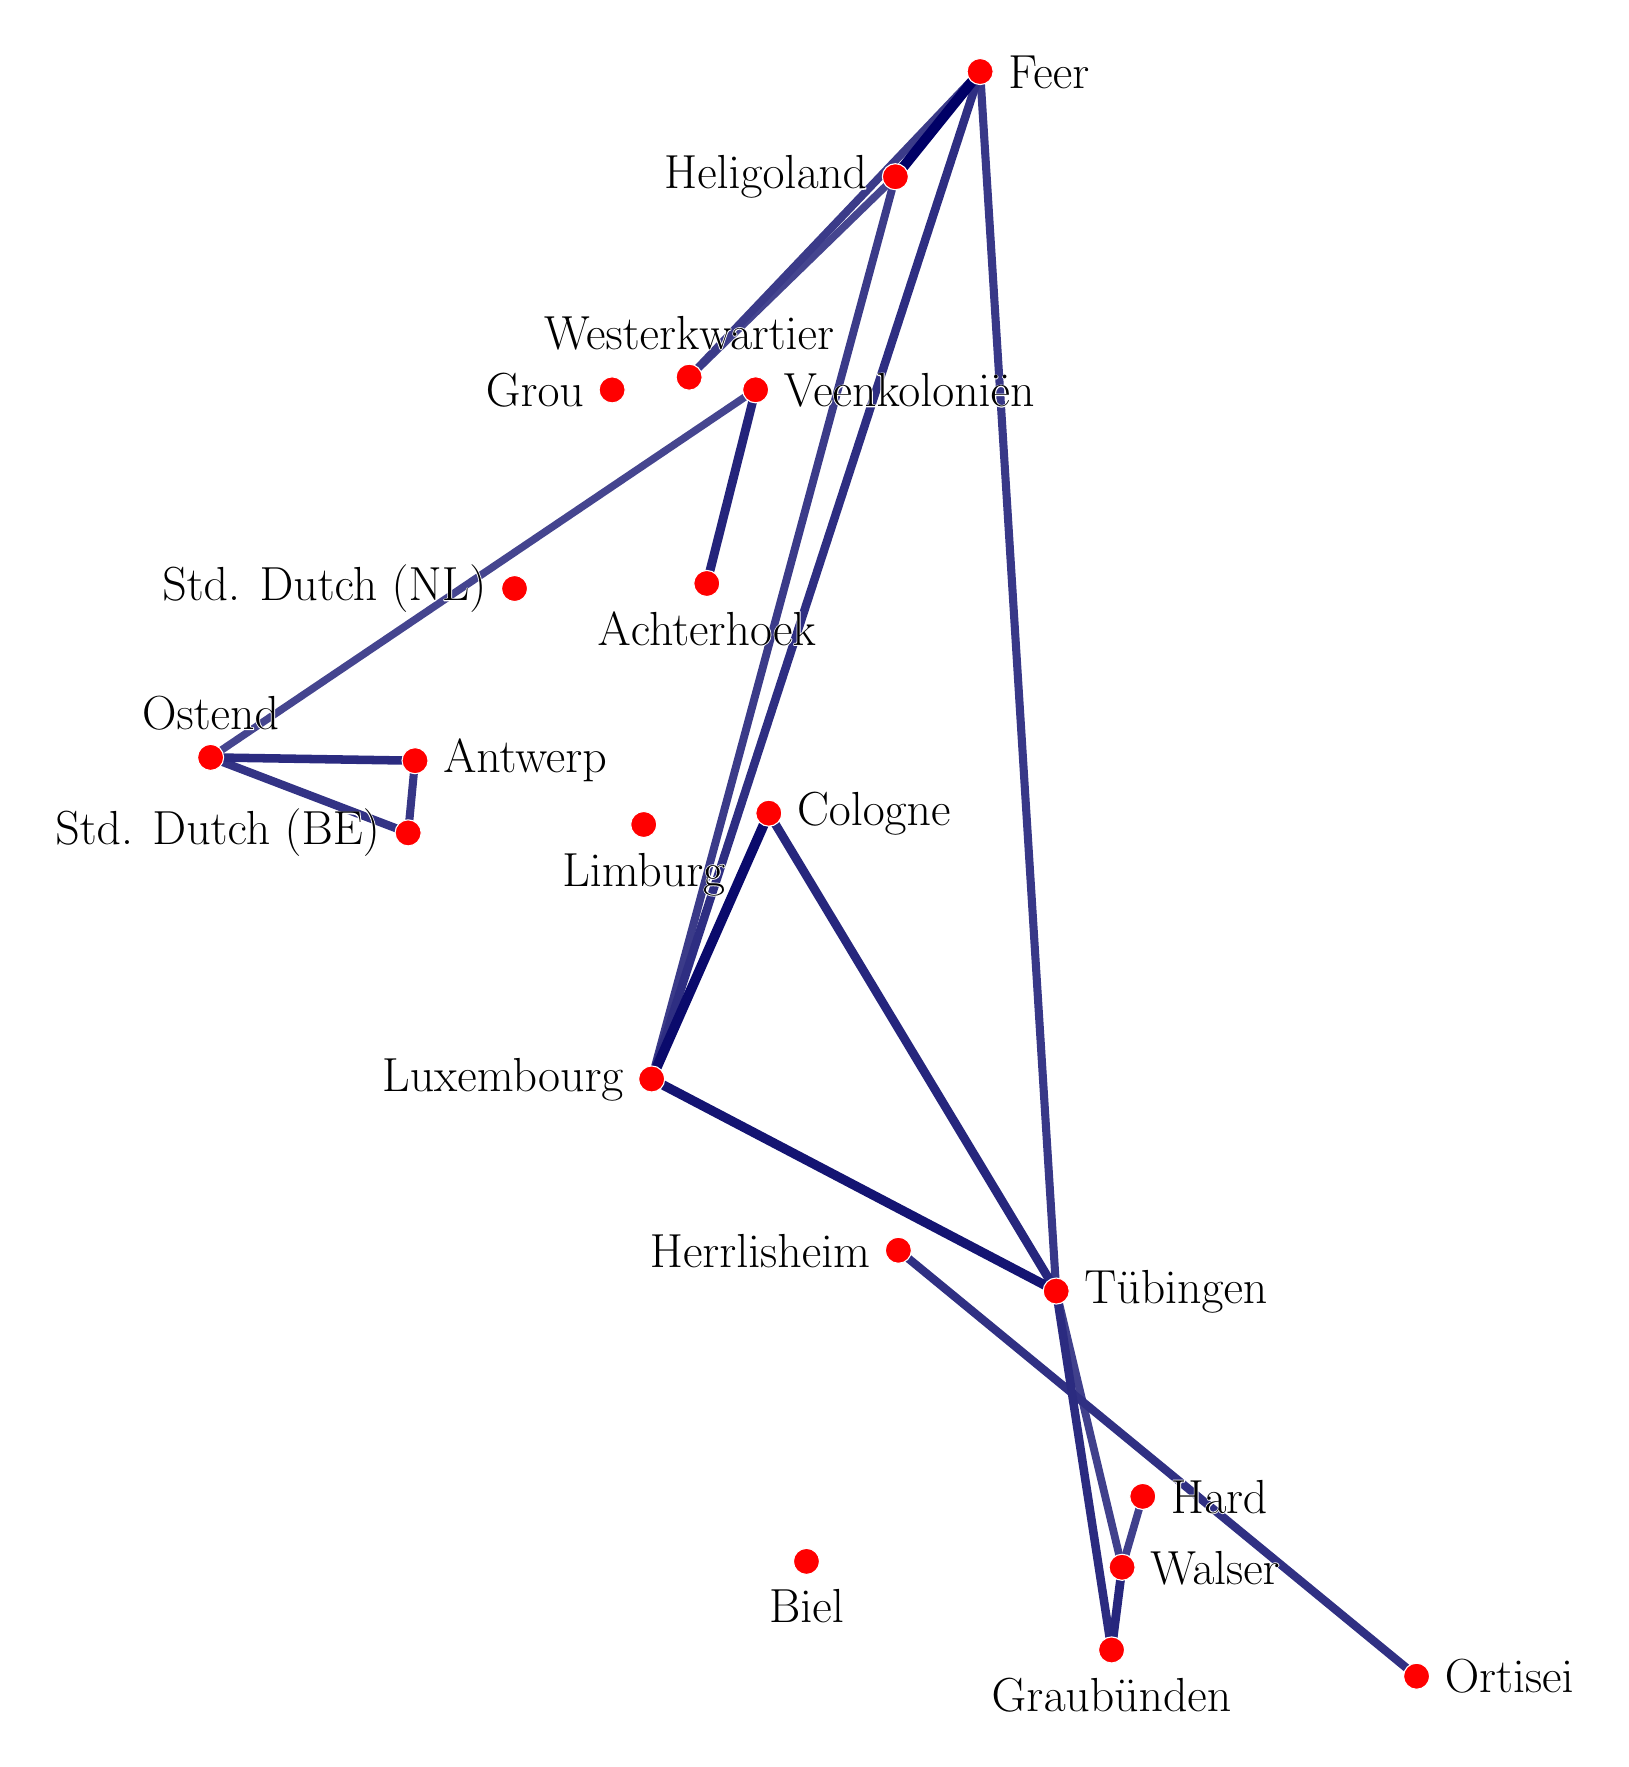
\begin{tikzpicture}[scale=2.5, dot/.style={draw=white, circle, minimum size=8pt, fill=red}, doculect/.style={inner sep=1em}]

% Establish doculect coordinates.
\node (StdDutchBE) at (3.0449999999999995, 50.85) {};
\node (Veenkolonien) at (4.809798, 53.10041999999999) {};
\node (Achterhoek) at (4.561668999999999, 52.11667) {};
\node (Herrlisheim) at (5.5347599999999995, 48.730059999999995) {};
\node (Ostend) at (2.0416689999999997, 51.23333) {};
\node (Tuebingen) at (6.336469999999999, 48.5229) {};
\node (StdDutchNL) at (3.5854000000000004, 52.091) {};
\node (Heligoland) at (5.519696000000001, 54.1825) {};
\node (Feer) at (5.949999999999999, 54.71666999999999) {};
\node (Walser) at (6.670999999999999, 47.12) {};
\node (Cologne) at (4.876669, 50.95) {};
\node (Ortisei) at (8.166668999999999, 46.56667) {};
\node (Antwerp) at (3.08, 51.21667) {};
\node (Luxembourg) at (4.281669, 49.6) {};
\node (Grou) at (4.0809999999999995, 53.1) {};
\node (Westerkwartier) at (4.47209, 53.16444) {};
\node (Hard) at (6.776, 47.48) {};
\node (Biel) at (5.068, 47.15) {};
\node (Graubuenden) at (6.617554999999999, 46.70013) {};
\node (Limburg) at (4.241419, 50.8925) {};

% Draw similarity lines.
\draw[line width=0.9527020372028397mm, color=black!60!blue!73](Heligoland.center) -- (Westerkwartier.center);
\draw[line width=0.9535776295242586mm, color=black!60!blue!73](Ostend.center) -- (Veenkolonien.center);
\draw[line width=0.9767958664187736mm, color=black!60!blue!75](Hard.center) -- (Walser.center);
\draw[line width=0.9869147714398687mm, color=black!60!blue!75](Tuebingen.center) -- (Walser.center);
\draw[line width=1.007626242662836mm, color=black!60!blue!77](Heligoland.center) -- (Luxembourg.center);
\draw[line width=1.0120956574884983mm, color=black!60!blue!77](Feer.center) -- (Westerkwartier.center);
\draw[line width=1.0265501870572231mm, color=black!60!blue!78](Feer.center) -- (Tuebingen.center);
\draw[line width=1.0271345479882565mm, color=black!60!blue!79](Antwerp.center) -- (StdDutchBE.center);
\draw[line width=1.048146344757306mm, color=black!60!blue!80](StdDutchBE.center) -- (Ostend.center);
\draw[line width=1.0612100318996298mm, color=black!60!blue!81](Herrlisheim.center) -- (Ortisei.center);
\draw[line width=1.0737177647017526mm, color=black!60!blue!82](Feer.center) -- (Luxembourg.center);
\draw[line width=1.0819051785131646mm, color=black!60!blue!83](Graubuenden.center) -- (Tuebingen.center);
\draw[line width=1.0832074930085054mm, color=black!60!blue!83](Antwerp.center) -- (Ostend.center);
\draw[line width=1.1135054560492381mm, color=black!60!blue!85](Cologne.center) -- (Tuebingen.center);
\draw[line width=1.11740837215337mm, color=black!60!blue!85](Graubuenden.center) -- (Walser.center);
\draw[line width=1.1263378556148649mm, color=black!60!blue!86](Achterhoek.center) -- (Veenkolonien.center);
\draw[line width=1.1975176667356227mm, color=black!60!blue!92](Luxembourg.center) -- (Tuebingen.center);
\draw[line width=1.2584925369920634mm, color=black!60!blue!96](Cologne.center) -- (Luxembourg.center);
\draw[line width=1.3mm, color=black!60!blue!100](Feer.center) -- (Heligoland.center);

% Mark the locations with circles and labels.
\node[dot] at (Antwerp.center) {};
\node[doculect, right] at (Antwerp.center) {\contour{white}{\LARGE Antwerp}};
\node[dot] at (Feer.center) {};
\node[doculect, right] at (Feer.center) {\contour{white}{\LARGE Feer}};
\node[dot] at (Herrlisheim.center) {};
\node[doculect, left] at (Herrlisheim.center) {\contour{white}{\LARGE Herrlisheim}};
\node[dot] at (Grou.center) {};
\node[doculect, left] at (Grou.center) {\contour{white}{\LARGE Grou}};
\node[dot] at (Achterhoek.center) {};
\node[doculect, below] at (Achterhoek.center) {\contour{white}{\LARGE Achterhoek}};
\node[dot] at (Walser.center) {};
\node[doculect, right] at (Walser.center) {\contour{white}{\LARGE Walser}};
\node[dot] at (Ortisei.center) {};
\node[doculect, right] at (Ortisei.center) {\contour{white}{\LARGE Ortisei}};
\node[dot] at (Luxembourg.center) {};
\node[doculect, left] at (Luxembourg.center) {\contour{white}{\LARGE Luxembourg}};
\node[dot] at (Biel.center) {};
\node[doculect, below] at (Biel.center) {\contour{white}{\LARGE Biel}};
\node[dot] at (Graubuenden.center) {};
\node[doculect, below] at (Graubuenden.center) {\contour{white}{\LARGE Graub\"{u}nden}};
\node[dot] at (StdDutchNL.center) {};
\node[doculect, left] at (StdDutchNL.center) {\contour{white}{\LARGE Std. Dutch (NL)}};
\node[dot] at (Westerkwartier.center) {};
\node[doculect, above] at (Westerkwartier.center) {\contour{white}{\LARGE Westerkwartier}};
\node[dot] at (Hard.center) {};
\node[doculect, right] at (Hard.center) {\contour{white}{\LARGE Hard}};
\node[dot] at (Veenkolonien.center) {};
\node[doculect, right] at (Veenkolonien.center) {\contour{white}{\LARGE Veenkoloni\"{e}n}};
\node[dot] at (StdDutchBE.center) {};
\node[doculect, left] at (StdDutchBE.center) {\contour{white}{\LARGE Std. Dutch (BE)}};
\node[dot] at (Heligoland.center) {};
\node[doculect, left] at (Heligoland.center) {\contour{white}{\LARGE Heligoland}};
\node[dot] at (Tuebingen.center) {};
\node[doculect, right] at (Tuebingen.center) {\contour{white}{\LARGE T\"{u}bingen}};
\node[dot] at (Cologne.center) {};
\node[doculect, right] at (Cologne.center) {\contour{white}{\LARGE Cologne}};
\node[dot] at (Ostend.center) {};
\node[doculect, above] at (Ostend.center) {\contour{white}{\LARGE Ostend}};
\node[dot] at (Limburg.center) {};
\node[doculect, below] at (Limburg.center) {\contour{white}{\LARGE Limburg}};
\end{tikzpicture}
\end{document}
